\subsection{Структура и работа}
Web-приложение — это клиент-серверное приложение, в котором осуществляется взаимодействие клиента с сервером, за 
счет браузера, а сервером является веб-сервер, который принимает HTTP-запросы от клиента (браузера), и в свою очередь 
выдает HTTP-ответы вместе с HTML-страницей, изображением или какими-нибудь другими данными. Клиенты могут получить доступ
к веб-серверу по URL адресу необходимой им страницы.

Для веб-приложений на стороне сервера можно применять различные технологии и любые языки программирования. 
Для клиента-браузера же не важно на какой ОС оно работает, в этом заключается один из главных плюсов --
кроссплатформенность (Рис.1).
\begin{figure}[H]
  \centering
  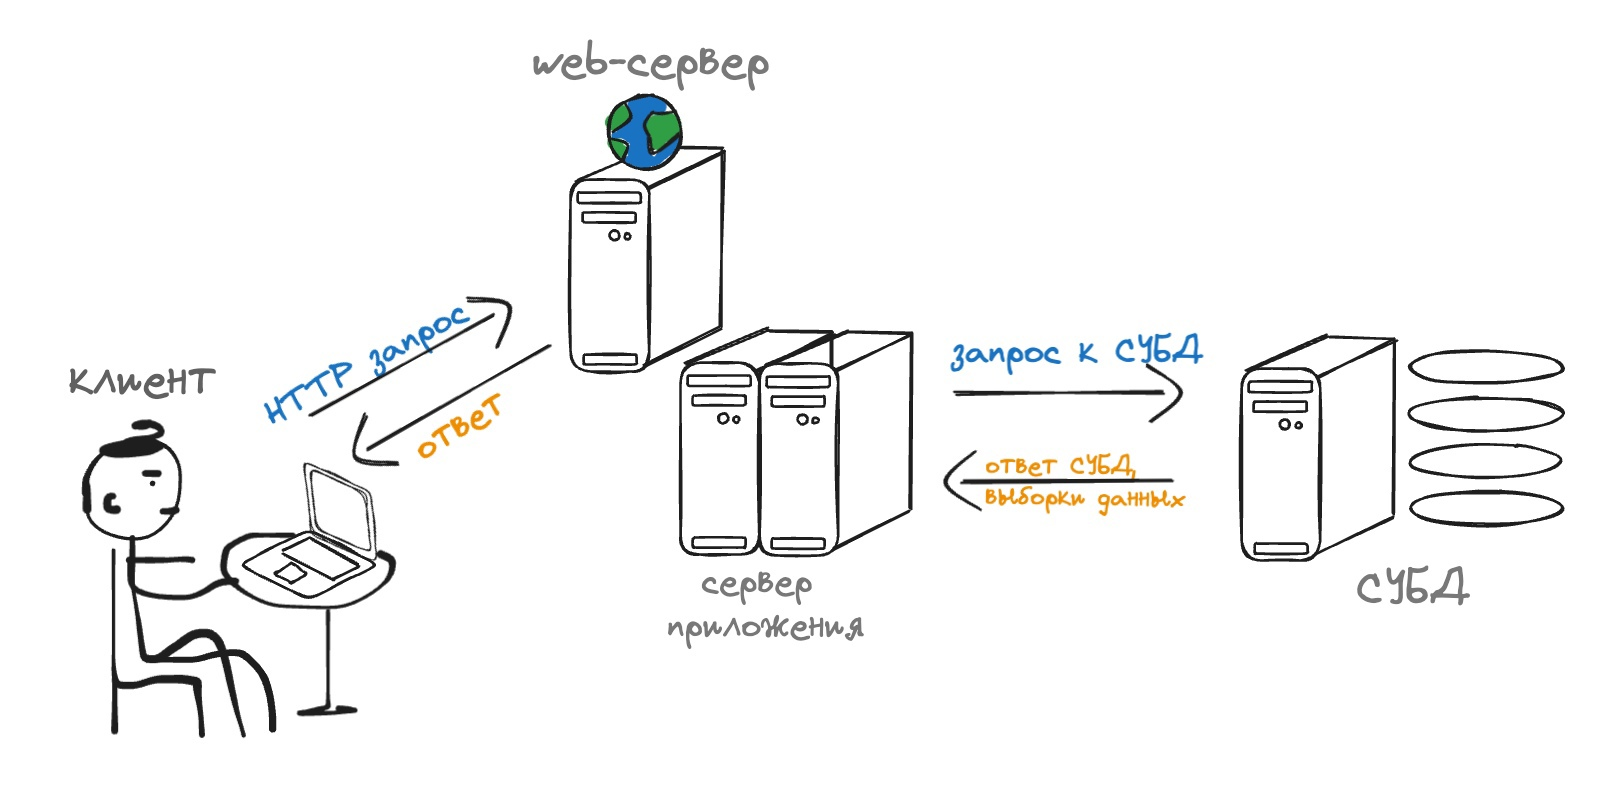
\includegraphics[width=1\textwidth]{pict/1}
  \caption{принцип обработки запросов приложением}
  \label{fig:1}
\end{figure}

Существует четыре общих уровня веб-приложений:
\begin{description}
\item[--]Представления (PL) имеет компоненты пользовательского интерфейса, которые показывают данные для пользователей, также
компоненты пользовательского процесса, которые задают взаимодействие с пользователем. PL предоставляет всю необходимую 
информацию клиентской стороне. Основная цель уровня представления - получить входные данные, обработать запросы пользователей,
отправить их в службу данных и показать результаты.

\item[--]Слой бизнес-логики BLL несет ответственность за надлежащий обмен данными между уровнем представления PL и уровнем обмена данными DAL, определяет логику бизнес-операций и правил. 

\item[--]Службы данных DSL передает данные, обработанные уровнем бизнес-логики, на уровень представления. Этот 
уровень гарантирует безопасность данных, изолируя бизнес-логику со стороны клиента.

\item[--]Доступа к данным DAL предлагает упрощенный доступ к данным, хранящимся в постоянных хранилищах (например XML). 
Уровень доступа к данным также управляет операциями CRUD - создание (C), чтение (R), обновление (U), удаление (D).

\end{description}
\begin{figure}[H]
  \centering
  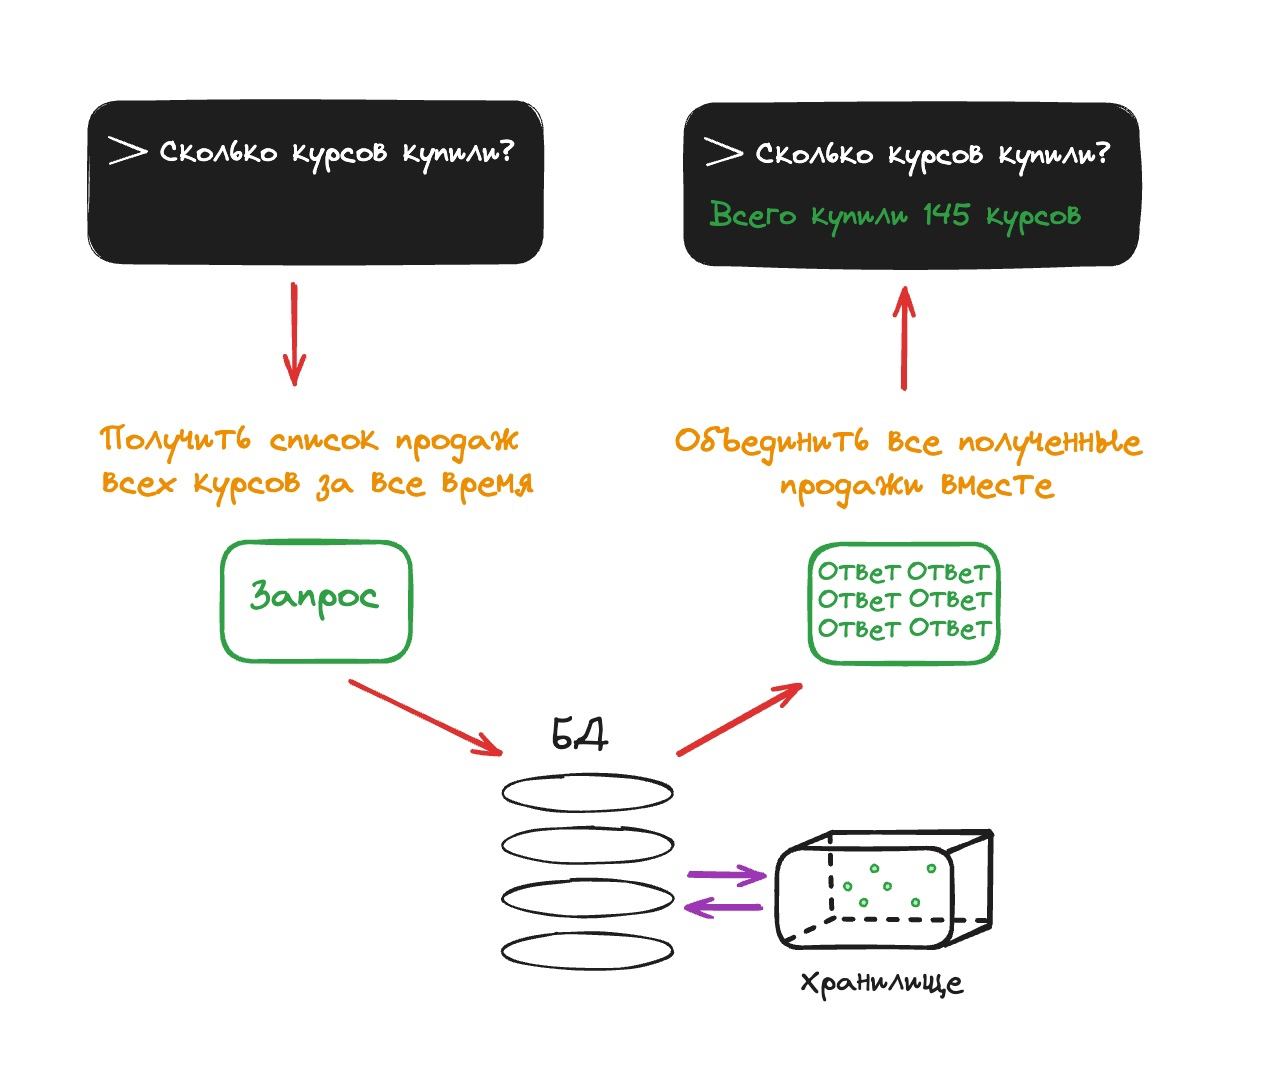
\includegraphics[width=1\textwidth]{pict/2}
  \caption{принцип взаимодействия уровней приложения}
  \label{fig:2}
\end{figure}

Чтобы приложение корректно и безопасно функционировало, необходимо, чтобы на каждом уровне
была обеспечена безопасность передаваемых данных и минимизирована возможность использования особенностей каждого уровня,
в качестве канала получения информации.


\newpage
\subsection{Уязвимости}
При работе с фреймворком разработчик используя функционал чаще всего
ограничивается знанием смысла работы какой-либо функции и ее параметров, не заглядывая внутрь 
нее, не зная всех деталей ее работы. Это большой плюс для разработчика, потому что с помощью
данной «абстракции», он может сконцентрироваться на решение своей задачи, не углубляясь
в ненужные подробности.

Большинство разработчиков не думает о безопасности работы приложения и данных, которыми 
оно оперирует, и тем более не считают это основной задачей, поэтому, если рассматривать
такое качество фреймворка как безопасность, то тем он будет лучше, чем больше будет 
предусматривать и закрывать возможные дыры в безопасности -- уязвимости.

На момент 2024 года такая организация как OWASP (Открытый проект обеспечения безопасности web-приложений) выделила следующие 
популярные уязвимости:
\begin{description}
  \item[--] нарушение контроля доступа;
  \item[--] недочёты криптографии;
  \item[--] инъекции;
  \item[--] небезопасный дизайн;
  \item[--] небезопасная конфигурация;
  \item[--] использование уязвимых или устаревших компонентов;
  \item[--] ошибки идентификации и аутентификации;
\end{description}

\textbf{Нарушение контроля целостности}

Это набор уязвимостей, при которых система плохо контролирует уровни доступа к информации или к своей функциональности.
Из-за этого злоумышленники могут пользоваться функциями, к которым не должны иметь доступа.
Если  веб-приложение, где каждая учётная запись имеет разные права доступа слабо защищено, злоумышленник
может модифицировать запросы или параметры URL, чтобы получить доступ к данным, на которые у него нет права.

\textbf{Недочеты криптографии}

Это уязвимости, связанные с неправильной настройкой и использованием криптографических методов 
для защиты данных. Это может быть недостаточная длина ключей, ненадёжные условия их хранения, использование устаревших 
алгоритмов и другие ошибки в криптографической реализации.

\textbf{Инъекции}

Данный вид уязвимостей -- пользовательский ввод с вредоносным кодом. Инъекции позволяют злоумышленникам внедрять свой вредоносный код 
на сервер и выполнять его. Результат -- потеря данных, кража данных или повреждение системы.

\textbf{Небезопасный дизайн}

Широкая категория уязвимостей, впервые появившаяся в последней версии OWASP Top Ten. Уязвимости этой категории возникают 
потому, что сама логика работы приложения может позволять использовать существующие функции в качестве уязвимостей.

\textbf{Небезопасная конфигурация} 

Это случаи, когда настройки приложения, сервера, базы данных или других компонентов системы 
не являются безопасными. К этому можно отнести ненадёжные или отсутствующие настройки аутентификации, 
авторизации и доступа, например отсутствие защиты от перебора пароля.

\textbf{Использование уязвимых компонентов}

К этому типу уязвимостей относят случаи, когда веб-приложение использует сторонние фреймворки, библиотеки, плагины или 
другие компоненты, которые имеют выявленные дефекты безопасности. У злоумышленников даже есть автоматизированные инструменты,
которые помогают находить неправильно сконфигурированные системы


\textbf{Ошибки идентификации и аутентификации}

Слабые пароли, недостаточная проверка подлинности, неэффективные системы учёта сеансов, все ошибки, которые могут возникнуть
из-за недостаточно безопасной реализации идентификации и аутентификации пользователя в системе.
   
\vspace{2mm}
Можно ли предотвратить реализацию большей части этих уязвимостей, если при разработке использовать определенные фреймворки, а может 
вообще что-то может быть обработано на уровне языка. В последующей своей работе, я рассмотрю самые популярные фреймворки для разработки
web-приложений и попробую проанализировать, какие базовые критерии безопасности они предусматривают. 